En este apartado se describirá el proceso de despliegue de la aplicación, detallando los componentes y servicios necesarios para su correcto funcionamiento. 
Se presentará un diagrama de despliegue que ilustrará la arquitectura de la aplicación y la distribución de los componentes en el entorno de ejecución. 

El despliegue de la aplicación se ha realizado en una máquina virtual (VM) de Azure con las siguientes características:
\begin{itemize}
    \item \textbf{Sistema Operativo}: Ubuntu 20.04 LTS.
    \item \textbf{Procesador}: 2 núcleos.
    \item \textbf{Memoria RAM}: 4 GB.
    \item \textbf{Discos de datos}: 4.
    \item \textbf{E/S máxima}: 1280 MB/s.
    \item \textbf{Almacenamiento local}: 8 GB.
    \item \textbf{Red}: IP pública y DNS asociado.
\end{itemize}

Para desplegar la aplicación, se han seguido los siguientes pasos:
\begin{enumerate}
    \item \textbf{Crear la máquina virtual en Azure}: Se ha creado una máquina virtual en Azure con las características mencionadas anteriormente. 
    Además, es necesario crear un grupo de recursos y una red virtual para la máquina virtual.

    \item \textbf{Contenedores Docker}: Se ha utilizado Docker para contenerizar la aplicación y facilitar su despliegue. 
    Para facilitar la tarea se ha configurado integración continua con GitHub Actions, de forma que cada vez que se realiza un \textit{pull-request} a la rama principal del repositorio, se construyen y despliegan los contenedores en la máquina virtual de Azure.
    Se han creado dos contenedores:
    \begin{itemize}
        \item \textbf{webapp}: Contiene la interfaz de usuario de la aplicación, implementada en React. Expuesto en el puerto 3000.
        \item \textbf{restapi}: Contiene la API REST del sistema, implementada en Node.js. Expuesto en el puerto 5001 para HTTP y 5002 para HTTPS.
    \end{itemize}

    \item \textbf{Configuración de Nginx}: Se ha configurado Nginx como servidor web inverso para redirigir las peticiones a los contenedores correspondientes.
    Este paso es necesario para poder acceder a la aplicación desde un navegador web y garantizar la seguridad de las comunicaciones con HTTPS.
    Se divide en dos partes:
    \begin{itemize}
        \item \textbf{Obtención de certificado SSL}: Se ha utilizado Certbot para obtener un certificado SSL gratuito de Let's Encrypt y habilitar el protocolo HTTPS en la aplicación.
        \item \textbf{Configuración de Nginx}: Se ha configurado Nginx para redirigir las peticiones HTTP y HTTPS a los contenedores webapp y restapi, respectivamente.
    \end{itemize}

    \item \textbf{Configuración de la base de datos}: Se ha utilizado MongoDB Atlas como base de datos para la aplicación. 
    Es necesario configurar la base de datos para que la API REST en el entorno de produción pueda conectarse a ella y almacenar los datos de la aplicación.

    \item \textbf{Docker Compose}: Se ha utilizado Docker Compose para orquestar los contenedores de la aplicación y facilitar su despliegue en la máquina virtual de Azure.
    Se ha creado un archivo \textit{docker-compose.yml} que define los servicios de la aplicación y sus configuraciones.

\end{enumerate}

Debido a los costos asociados al uso de la máquina virtual en Azure, se ha optado por mantener la máquina virtual apagada cuando no se está utilizando la aplicación.
Está configurada para apagarse automáticamente a las 22:00 y encenderse manualmente cuando se necesita acceder a la aplicación.


En la \coloredUnderline{\hyperlink{fig:6_6_Diagrama-Despliegue}{Figura \ref*{fig:6_6_Diagrama-Despliegue}: \nameref*{fig:6_6_Diagrama-Despliegue}}} se muestra el diagrama de despliegue de la aplicación.
\begin{figure}[H]
    \hypertarget{fig:6_6_Diagrama-Despliegue}{}
    \centering
    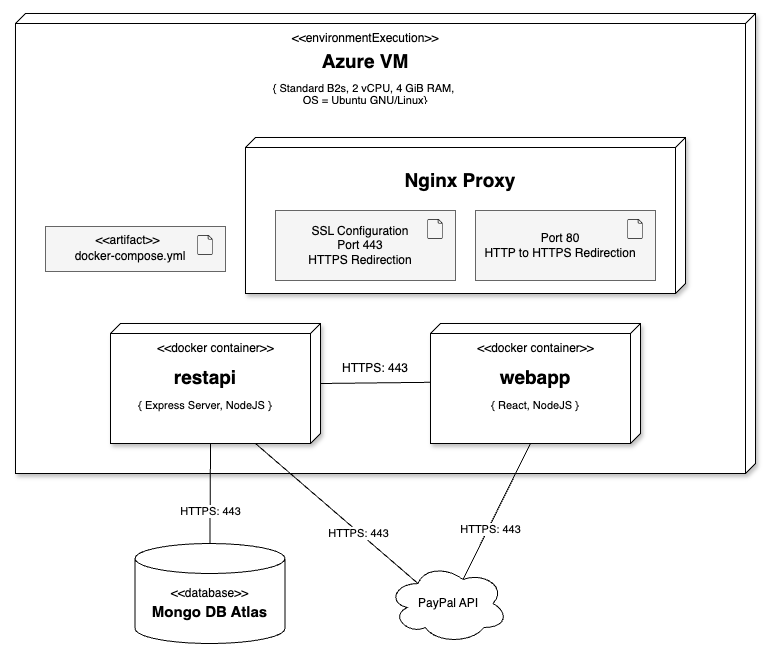
\includegraphics[width=0.8\linewidth]{figures/6-Analisis/6-Clases/6_5-Deployment.png}
    \caption{Diagrama de Despliegue de la Aplicación}
    \label{fig:6_6_Diagrama-Despliegue}
\end{figure}